% GeneticWing, A0 portrait poster. Build: lualatex geneticwing_poster.tex (twice), after
%   PYTHONPATH=src python docs/poster/make_figures.py
% \pending{...} typesets a value still waiting for a run (orange, dashed box).
\documentclass{article}
\usepackage[paperwidth=841mm,paperheight=1189mm,margin=0mm]{geometry}
\usepackage{lmodern}
\usepackage{fontspec}
\setmainfont{Segoe UI}[BoldFont={Segoe UI Bold},ItalicFont={Segoe UI Italic},BoldItalicFont={Segoe UI Bold Italic}]
\newfontfamily\lightfont{Segoe UI Light}
\newfontfamily\semifont{Segoe UI Semibold}
\usepackage{xcolor,graphicx,tikz,qrcode,enumitem,array,booktabs}
\usetikzlibrary{positioning,arrows.meta,calc,fit,backgrounds,shapes.misc}
\usepackage[hidelinks]{hyperref}
\pagestyle{empty}
\setlength{\parindent}{0pt}
\setlength{\parskip}{0.45em}
\AtBeginDocument{\raggedright}

% Colours: the entities keep the figures' colours.
\definecolor{ink}{HTML}{0B0B0B}
\definecolor{ink2}{HTML}{52514E}
\definecolor{rule}{HTML}{2A78D6}
\definecolor{ga}{HTML}{1BAF7A}
\definecolor{gen}{HTML}{EB6834}
\definecolor{motor}{HTML}{8A8F98}
\definecolor{navy}{HTML}{0D2A4F}
\definecolor{sky}{HTML}{EEF4FC}
\definecolor{paper}{HTML}{FFFFFF}
\definecolor{line}{HTML}{E4E3DF}
\pagecolor{paper}
\color{ink}

% Type scale (A0, read from 1.5 m).
\renewcommand\normalsize{\fontsize{27}{36}\selectfont}
\renewcommand\small{\fontsize{22}{29}\selectfont}
\renewcommand\footnotesize{\fontsize{19}{25}\selectfont}
\renewcommand\large{\fontsize{34}{42}\selectfont}
\renewcommand\Large{\fontsize{44}{54}\selectfont}
\renewcommand\huge{\fontsize{60}{70}\selectfont}
\renewcommand\Huge{\fontsize{120}{130}\selectfont}
\normalsize
\setlist{leftmargin=1.1em,itemsep=0.25em,topsep=0.3em,parsep=0pt,label={\color{gen}\textbullet}}

\newcounter{sec}
\newcommand\sect[1]{%
  \stepcounter{sec}\par\vspace{0.8em}%
  \begin{tikzpicture}
    \node[circle,fill=navy,text=white,minimum size=1.55em,inner sep=0pt,font=\semifont\large] (n) {\thesec};
    \node[right=0.45em of n,anchor=west,font=\semifont\Large,text=navy] {#1};
  \end{tikzpicture}\par\vspace{-0.15em}%
  {\color{gen}\rule{\linewidth}{4pt}}\par\vspace{0.3em}}
\newcommand\fig[2][\linewidth]{\par{\centering\includegraphics[width=#1]{figures/#2}\par}}
\newcommand\figcap[1]{{\small\color{ink2}#1\par}}
\newcommand\key[1]{{\semifont\color{navy}#1}}
\newcommand\pending[1]{\tikz[baseline=(p.base)]\node[draw=gen,dashed,line width=2pt,rounded corners=4pt,
  text=gen,inner sep=6pt,font=\semifont](p){#1};}

\begin{document}
\noindent\begin{tikzpicture}[remember picture,overlay]
  \fill[navy] (current page.north west) rectangle ([yshift=-150mm]current page.north east);
\end{tikzpicture}\par
\vspace*{8mm}
\noindent\hspace*{25mm}%
\begin{minipage}[t]{640mm}
  {\color{white}\fontsize{116}{122}\selectfont\semifont GeneticWing\par}
  \vspace{4mm}
  {\color{white}\lightfont\fontsize{50}{60}\selectfont A sailplane that learns how to climb in thermals\par}
  \vspace{7mm}
  {\color{white!80!navy}\fontsize{30}{36}\selectfont Clément Dumeril \quad\textbar\quad
   simulation study, 2026 \quad\textbar\quad clementdumeril.github.io/GeneticWing\par}
\end{minipage}%
\hfill
\begin{minipage}[t]{130mm}\vspace{2mm}\raggedleft
  \colorbox{white}{\qrcode[height=78mm,nolink]{https://clementdumeril.github.io/GeneticWing/}}\\[2mm]
  {\color{white!80!navy}\footnotesize fly it in 3D in your browser}
\end{minipage}\hspace*{25mm}

\vspace{6mm}
% ---------------------------------------------------------------- hero image and headline numbers
\hspace*{25mm}\begin{tikzpicture}
  \node[inner sep=0pt,anchor=north west] (hero) at (0,0) {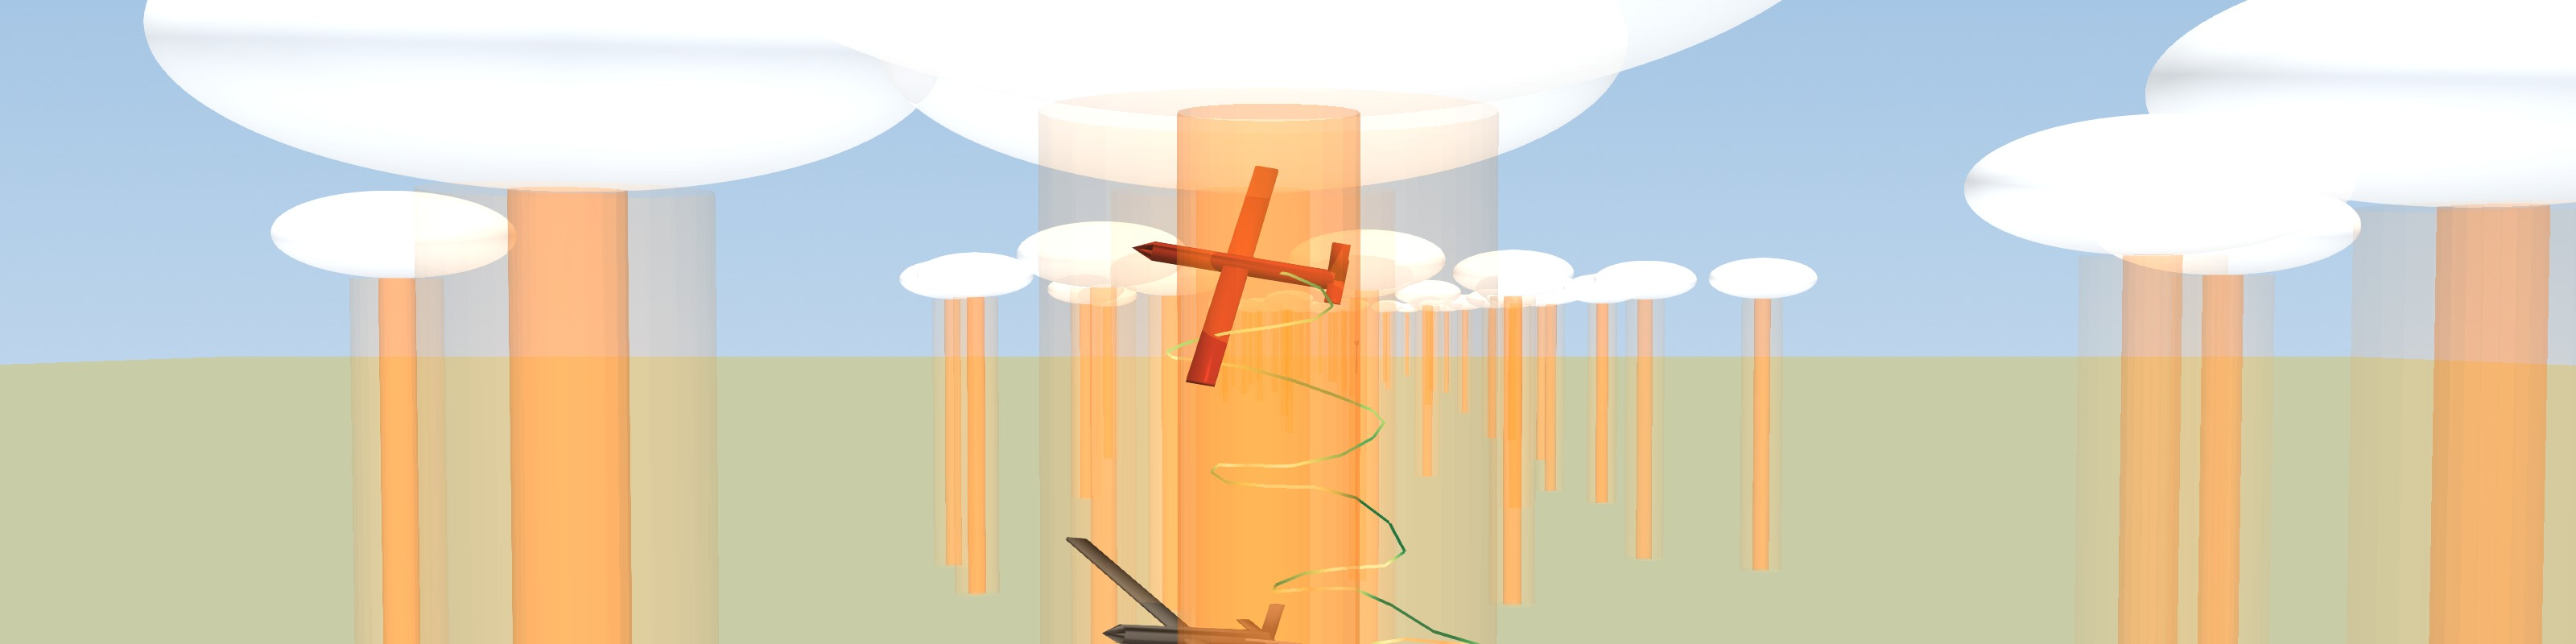
\includegraphics[width=791mm]{figures/hero.jpg}};
  \node[anchor=south west,fill=white,fill opacity=0.88,text opacity=1,inner sep=10pt,rounded corners=6pt,
        text width=300mm,font=\small] at ([xshift=10mm,yshift=10mm]hero.south west)
    {\semifont Simulated flight.\ \normalfont The red sailplane plans every climb; the grey one follows the
     standard circling rule. Same thermals, same decisions about which thermal to take.
     The trail turns green where it climbs.};
  \foreach \v/\t/\c [count=\i] in {
      {1.7\texttimes}/{faster climbs than\\the circling rule}/gen,
      {0.24 s}/{to plan a climb,\\56\texttimes{} faster than search}/gen,
      {+70\,\%}/{climb rate on 64 tasks\\never seen in training}/gen} {
    \node[anchor=north east,fill=white,fill opacity=0.92,text opacity=1,rounded corners=6pt,inner sep=9pt,
          text width=150mm,align=left] at ([xshift=-10mm,yshift={-8mm-(\i-1)*63mm}]hero.north east)
      {{\color{\c}\fontsize{64}{66}\selectfont\semifont \v}\par\vspace{1mm}{\small\color{ink}\t}};
  }
\end{tikzpicture}

% ---------------------------------------------------------------- how it works
\vspace{8mm}
\hspace*{25mm}\begin{minipage}{791mm}
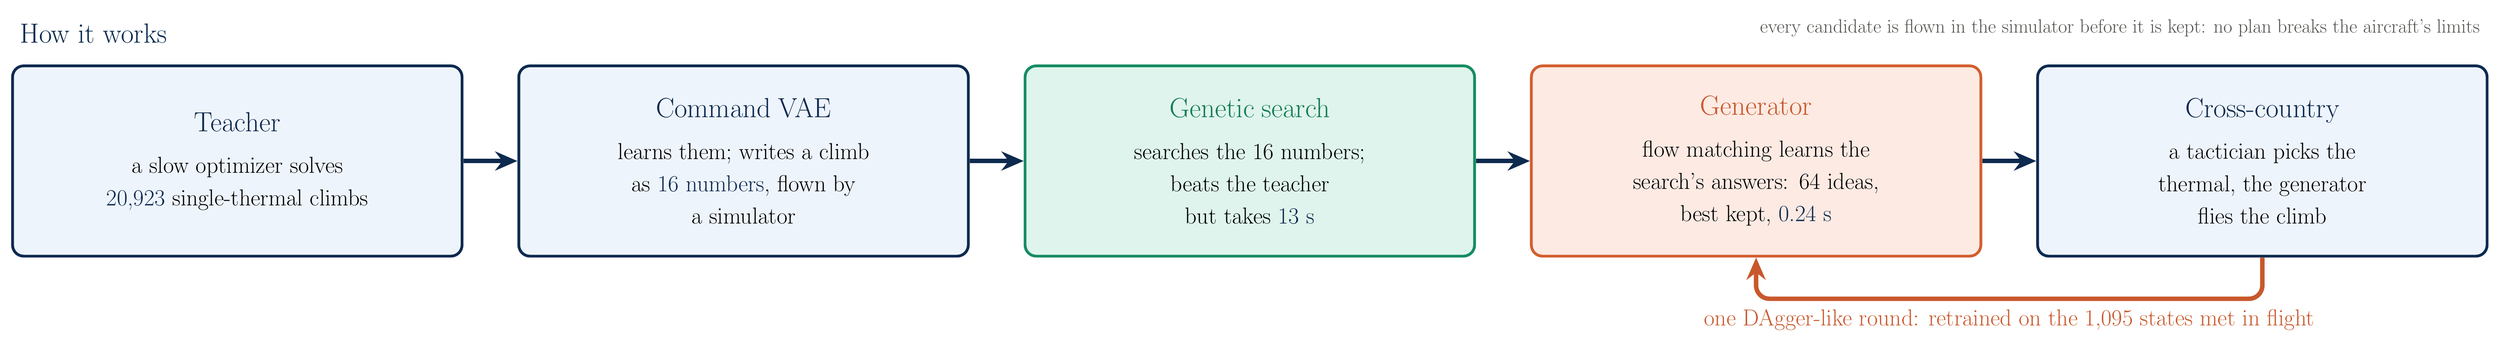
\begin{tikzpicture}[
    stage/.style={draw=navy,line width=2.5pt,rounded corners=10pt,fill=sky,text width=136mm,minimum height=60mm,
                 align=center,inner sep=8pt,font=\small},
    flow/.style={-{Stealth[length=7mm,width=6mm]},line width=4pt,color=navy}]
  \node[stage] (t) {{\semifont\large\color{navy} Teacher}\\[3mm]a slow optimizer solves\\\key{20,923} single-thermal climbs};
  \node[stage,right=17mm of t] (v) {{\semifont\large\color{navy} Command VAE}\\[3mm]learns them; writes a climb\\as \key{16 numbers}, flown by\\a simulator};
  \node[stage,right=17mm of v,fill=ga!14,draw=ga!80!black] (g) {{\semifont\large\color{ga!70!black} Genetic search}\\[3mm]searches the 16 numbers;\\beats the teacher\\but takes \key{13 s}};
  \node[stage,right=17mm of g,fill=gen!14,draw=gen!90!black] (f) {{\semifont\large\color{gen!85!black} Generator}\\[3mm]flow matching learns the\\search's answers: 64 ideas,\\best kept, \key{0.24 s}};
  \node[stage,right=17mm of f] (x) {{\semifont\large\color{navy} Cross-country}\\[3mm]a tactician picks the\\thermal, the generator\\flies the climb};
  \foreach \a/\b in {t/v,v/g,g/f,f/x} \draw[flow] (\a) -- (\b);
  \draw[flow,gen!85!black,rounded corners=12pt] (x.south) -- ++(0,-13mm) -| node[pos=0.25,below,font=\small,text=gen!85!black]
     {one DAgger-like round: retrained on the 1,095 states met in flight} (f.south);
  \node[anchor=south west,font=\semifont\large,text=navy] at ([yshift=4mm]t.north west) {How it works};
  \node[anchor=south east,font=\footnotesize,text=ink2] at ([yshift=6mm]x.north east)
     {every candidate is flown in the simulator before it is kept: no plan breaks the aircraft's limits};
\end{tikzpicture}
\end{minipage}

% ---------------------------------------------------------------- three columns
\vspace{6mm}
\hspace*{25mm}%
\begin{minipage}[t]{249mm}
\sect{The problem}
A small motor-glider (SB-XC, \key{4.2\,kg}) can save its battery by climbing in thermals, columns of rising
air, like a glider pilot. But each thermal has a strong core, weak edges and sinking air around it, and it drifts
with the wind.
\begin{itemize}
  \item circle too wide: the aircraft misses the core;
  \item circle too tight: the inner wing stalls.
\end{itemize}
Planning the best circle is a hard, many-solution problem with the solutions sitting on the stall limit.
\fig{thermal.pdf}
\figcap{The thermal model used here (Allen, NASA 2006) on a real day: vertical air speed around the core.}

\sect{Why a learned space?}
The same genetic search, with the same time budget, does far better in the VAE's 16 learned numbers than in
hand-made descriptions of the commands, and beats the teacher it learned from.
\fig{learned_space.pdf}
\figcap{Energy gained in a 60\,s climb (higher is better), 49 test climbs. Grey: commands described by
knots, or raw.}

\sect{Honest limits}
\begin{itemize}
  \item Simulation only; the aircraft's polar is estimated. With 20\,\% more mass, the search's lead shrinks.
  \item Given 2 minutes per climb, a nonlinear MPC beats the genetic search; given 20\,s it solves half the climbs.
  \item On the windy day the blind generator lands out more often than the blind rule. Next: wind, then a flight test.
\end{itemize}
\end{minipage}%
\hspace{22mm}%
\begin{minipage}[t]{249mm}
\sect{As good as search, 56\texttimes{} faster}
The search is good but slow. A generator trained on its answers proposes 64 climbs, flies each one in the simulator
and keeps the best: the search's quality in a quarter of a second.
\fig{speed_quality.pdf}
\figcap{65 test climbs. One generator sample alone is not enough; 64 verified samples are.}

\sect{In a 20 km cross-country flight}
A tactician chooses which thermal to take; only the climbs differ. The generator climbs
\key{1.7\texttimes} faster than the circling rule and keeps it on tasks it has never seen.
\fig{climbs.pdf}
\figcap{Mean climb rate, 64 tasks of 20\,km each (MacCready 0.5). The DAgger-like round used the training tasks.}
\vspace{2mm}
\fig{barogram.pdf}
\figcap{One task: faster climbs, higher glides, 4 minutes earlier, no battery used.}
\end{minipage}%
\hspace{22mm}%
\begin{minipage}[t]{249mm}
\sect{Into a real day}
The thermals now come from a real weather forecast (DWD ICON-D2) over Issoudun, France, for three days of summer
2025. They are born, drift with the forecast wind and die.
\fig[0.9\linewidth]{weather_map.pdf}
\figcap{12 July 2025: forecast thermal strength, the thermals alive at mid-flight and one task.}

\sect{Flying blind}
A real pilot does not see the thermal. The blind pilots feel it through the variometer, estimate its centre and
strength with a Kalman filter (as ArduSoar does), and plan from that estimate.
\fig{weather_bars.pdf}
\figcap{48 tasks of 20\,km per day, MacCready 1. Hatched: blind. Without seeing the thermals, the rule needs the motor to find them (45\,kJ instead of 1). The generator, retrained on these weather thermals, needs \key{44\,\% less battery} than the blind rule on the cumulus day and 8\,\% less on the strong day. On the windy day it reaches the goal less often (69\,\% against 92\,\%).}

\end{minipage}

% ---------------------------------------------------------------- footer
\vfill
\hspace*{25mm}\begin{minipage}{791mm}
{\color{line}\rule{\linewidth}{2pt}}\par\vspace{2mm}
\footnotesize\color{ink2}
Allen, Updraft model for autonomous soaring, NASA/TM-2006-214382 \textbullet{}
Morando et al., flatness-based glide planning, ICRA 2025 \textbullet{}
Lipman et al., Flow matching, ICLR 2023 \textbullet{}
Ross et al., DAgger, AISTATS 2011 \textbullet{}
Forecasts: DWD ICON-D2 via Open-Meteo (CC BY 4.0) \textbullet{}
Computed on the Savio cluster (UC Berkeley).
\end{minipage}
\vspace*{18mm}
\end{document}
